\documentclass{article}
\usepackage[a4paper, margin=1in]{geometry}
\usepackage{amsmath}
\usepackage{amssymb}
\usepackage{fancyhdr}
\usepackage{graphicx}
\usepackage{tikz}
\usepackage{circuitikz} % Use the dedicated circuitikz package for circuits
\usetikzlibrary{arrows.meta, positioning, decorations.pathmorphing, patterns}

% --- Header and Footer ---
\pagestyle{fancy}
\fancyhf{}
\rhead{SHM in Physics}
\lhead{Generated by Gemini}
\cfoot{\thepage}

\title{\textbf{Problems on Simple Harmonic Motion in Physical Fields}}
\author{Generated by Gemini}
\date{\today}

\begin{document}

\maketitle
\tableofcontents
\newpage

\section{SHM in Electric and Magnetic Fields}

\subsection{Problem 1: Dipole in a Uniform Electric Field}
\subsubsection*{Problem Statement}
An electric dipole consists of two charges $+q$ and $-q$ separated by a distance $d$. It has a dipole moment of magnitude $p=qd$ and a moment of inertia $I$. The dipole is placed in a uniform electric field $\vec{E}$ and is slightly displaced from its stable equilibrium position by a small angle $\theta$. Show that the dipole executes simple harmonic motion and find its period of oscillation.

\begin{center}
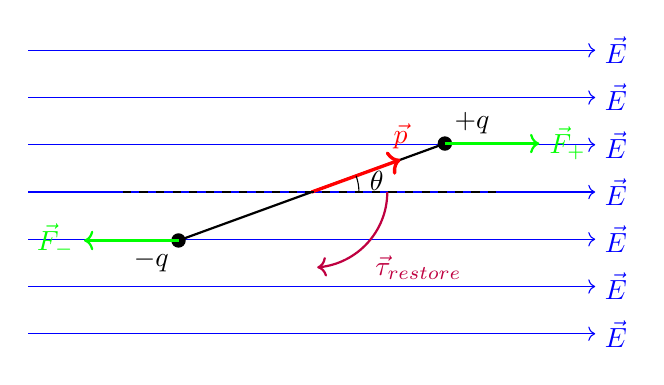
\begin{tikzpicture}[scale=1.2]
    % Uniform E-field
    \foreach \y in {-1.5, -1, -0.5, 0, 0.5, 1, 1.5}
    \draw[->, blue] (-3, \y) -- (3, \y) node[right] {$\vec{E}$};

    % Dipole
    \def\angle{20}
    \draw[thick] ({-1.5*cos(\angle)}, {-1.5*sin(\angle)}) -- ({1.5*cos(\angle)}, {1.5*sin(\angle)});
    \filldraw ({1.5*cos(\angle)}, {1.5*sin(\angle)}) circle (2pt) node[above right] {$+q$};
    \filldraw ({-1.5*cos(\angle)}, {-1.5*sin(\angle)}) circle (2pt) node[below left] {$-q$};
    \draw[->, very thick, red] (0,0) -- (\angle:1) node[above] {$\vec{p}$};
    
    % Forces creating torque
    \draw[->, green, thick] ({1.5*cos(\angle)}, {1.5*sin(\angle)}) -- ({1.5*cos(\angle)+1}, {1.5*sin(\angle)}) node[right] {$\vec{F}_+$};
    \draw[->, green, thick] ({-1.5*cos(\angle)}, {-1.5*sin(\angle)}) -- ({-1.5*cos(\angle)-1}, {-1.5*sin(\angle)}) node[left] {$\vec{F}_-$};

    % Angle and Torque
    \draw[dashed] (-2,0) -- (2,0);
    \draw (0.5,0) arc (0:\angle:0.5);
    \node at (\angle/2:0.7) {$\theta$};
    \draw[->, purple, thick, shorten >= 2pt] (0.8,0) arc (0:-90:0.8) node[midway, below right] {$\vec{\tau}_{restore}$};
\end{tikzpicture}
\end{center}

\subsubsection*{Explanation and Solution}
The torque $\vec{\tau}$ on an electric dipole in an electric field is given by $\vec{\tau} = \vec{p} \times \vec{E}$. The magnitude of this torque is $\tau = pE\sin\theta$. For a displacement from the stable equilibrium position ($\theta=0$), this torque acts to restore the dipole to alignment. We denote this restoring torque with a negative sign:
$$\tau = -pE\sin\theta$$
For simple harmonic motion, we use the small-angle approximation, $\sin\theta \approx \theta$ for small $\theta$:
$$\tau \approx -pE\theta$$
This is in the required form, $\tau = -\kappa\theta$, with the torsional constant $\kappa = pE$.
From Newton's second law for rotation, $\tau = I\alpha = I\frac{d^2\theta}{dt^2}$. Equating the two expressions for torque:
$$I\frac{d^2\theta}{dt^2} = -pE\theta \implies \frac{d^2\theta}{dt^2} + \left(\frac{pE}{I}\right)\theta = 0$$
This is the standard differential equation for SHM. By comparison, the angular frequency is $\omega = \sqrt{\frac{pE}{I}}$. The period of oscillation $T$ is $T = 2\pi/\omega$.
$$T = 2\pi\sqrt{\frac{I}{pE}}$$

\hrulefill
\subsection{Problem 2: Current-Carrying Coil in a Magnetic Field}
\subsubsection*{Problem Statement}
A rectangular coil of $N$ turns, with side lengths $a$ and $b$, carries a current $I$. The coil is pivoted along an axis and placed in a uniform magnetic field $\vec{B}$ that is perpendicular to the pivot axis. The coil has a moment of inertia $I_{rot}$ about this axis. If the coil is rotated by a small angle $\theta$ from its stable equilibrium position and released, show that it oscillates with SHM and find its angular frequency.

\begin{center}
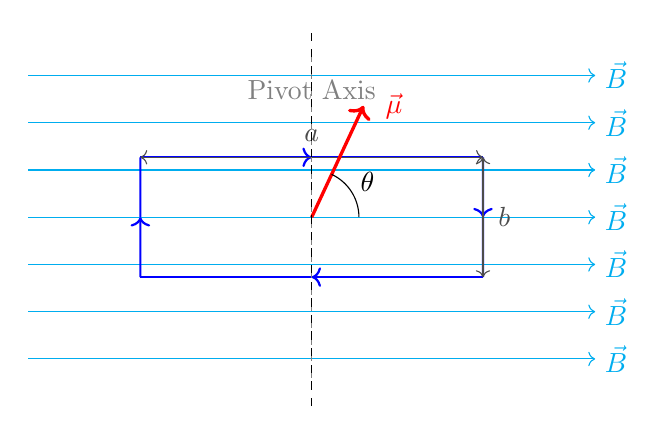
\begin{tikzpicture}[scale=1.2]
    % Magnetic Field Lines
    \foreach \y in {-1.5, -1, -0.5, 0, 0.5, 1, 1.5}
    \draw[->, cyan] (-3, \y) -- (3, \y) node[right] {$\vec{B}$};
    
    % Coil (perspective view)
    \def\angle{25}
    \def\width{2}
    \def\height{1.5}

    % Coordinates for the rotated rectangle
    \coordinate (BL) at ({- \width * cos(\angle)}, {-\height * sin(\angle)});
    \coordinate (BR) at ({  \width * cos(\angle)}, {-\height * sin(\angle)});
    \coordinate (TR) at ({  \width * cos(\angle)}, { \height * sin(\angle)});
    \coordinate (TL) at ({- \width * cos(\angle)}, { \height * sin(\angle)});

    % Draw the coil outline with current arrows
    \draw[blue, thick, ->] (BL) -- ($(BL)!0.5!(TL)$); \draw[blue, thick] ($(BL)!0.5!(TL)$) -- (TL);
    \draw[blue, thick, ->] (TL) -- ($(TL)!0.5!(TR)$); \draw[blue, thick] ($(TL)!0.5!(TR)$) -- (TR);
    \draw[blue, thick, ->] (TR) -- ($(TR)!0.5!(BR)$); \draw[blue, thick] ($(TR)!0.5!(BR)$) -- (BR);
    \draw[blue, thick, ->] (BR) -- ($(BR)!0.5!(BL)$); \draw[blue, thick] ($(BR)!0.5!(BL)$) -- (BL);

    % Labels for dimensions
    \draw[<->, black!70] (BR) -- (TR) node[midway, right=2pt] {$b$};
    \draw[<->, black!70] (TL) -- (TR) node[midway, above=2pt] {$a$};
    
    % Pivot axis
    \draw[dashed, gray] (0,-1.7) -- (0,1.7) node[below=5pt] {Pivot Axis};

    % Magnetic Moment vector
    \draw[->, red, very thick] (0,0) -- ({90-\angle}:1.3) node[right=4pt] {$\vec{\mu}$};
    
    % Angle theta
    \draw[dashed] (0, -2) -- (0,2);
    \draw (0.5,0) arc (0:{90-\angle}:0.5);
    \node at ({(90-\angle)/2}:0.7) {$\theta$};
\end{tikzpicture}
\end{center}

\subsubsection*{Explanation and Solution}
A current-carrying coil in a magnetic field has a magnetic dipole moment $\vec{\mu}$ of magnitude $\mu = NIA$, where $A=ab$. The torque on the dipole is $\vec{\tau} = \vec{\mu} \times \vec{B}$, with magnitude $\tau = \mu B \sin\theta$. The restoring torque for a small displacement from equilibrium ($\theta=0$) is:
$$\tau = -\mu B \sin\theta$$
Using the small-angle approximation $\sin\theta \approx \theta$:
$$\tau \approx -(NIAB)\theta$$
This is a linear restoring torque. From Newton's second law for rotation, $\tau = I_{rot}\frac{d^2\theta}{dt^2}$:
$$I_{rot}\frac{d^2\theta}{dt^2} = -(NIAB)\theta \implies \frac{d^2\theta}{dt^2} + \left(\frac{NIAB}{I_{rot}}\right)\theta = 0$$
This is the SHM equation. The angular frequency of oscillation is:
$$\omega = \sqrt{\frac{NIAB}{I_{rot}}}$$

\newpage
\section{SHM in a Gravitational Field}

\subsection{Problem 3: Tunnel Through the Earth's Center}
\subsubsection*{Problem Statement}
Assume the Earth is a sphere of uniform density $\rho$, mass $M$, and radius $R$. A straight, frictionless tunnel is drilled along a diameter. A particle of mass $m$ is dropped into the tunnel from the surface. Show that the particle executes SHM and calculate the period of its motion.

\begin{center}
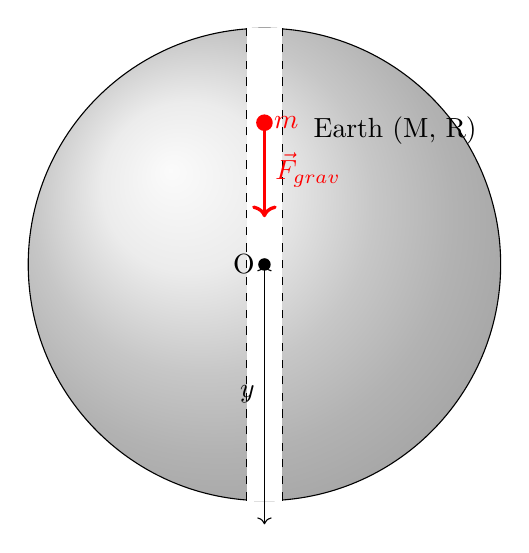
\begin{tikzpicture}[scale=1.5]
    % Earth
    \shade[ball color=gray!40!white, opacity=0.5] (0,0) circle (2cm);
    \draw (0,0) circle (2cm) node[above right=1.4cm and 0.5cm] {Earth (M, R)};

    % Tunnel
    \fill[white] (-0.15,-2) rectangle (0.15,2);
    \draw[dashed] (0.15, -2) -- (0.15, 2);
    \draw[dashed] (-0.15,-2) -- (-0.15, 2);
    
    % Center and Particle
    \fill (0,0) circle (1.5pt) node[left] {O};
    \coordinate (P) at (0, 1.2);
    \fill[red] (P) circle (2pt) node[right] {$m$};
    
    % Labels and Force Vector
    \draw[<->] (0,-2.2) -- (0,0) node[midway, left] {$y$};
    \draw[->, red, very thick] (P) -- (0, 0.4) node[midway, right] {$\vec{F}_{grav}$};
\end{tikzpicture}
\end{center}

\subsubsection*{Explanation and Solution}
Inside the Earth at a distance $y$ from the center, the gravitational force is due only to the mass enclosed within that radius, $M_{enc} = M (y^3/R^3)$. The gravitational force on the particle is:
$$F_g = -G \frac{M_{enc} m}{y^2} = -G \frac{(M y^3/R^3) m}{y^2} = -\left(\frac{GMm}{R^3}\right)y$$
This force is a linear restoring force. According to Newton's second law:
$$m\frac{d^2y}{dt^2} = -\left(\frac{GMm}{R^3}\right)y \implies \frac{d^2y}{dt^2} + \left(\frac{GM}{R^3}\right)y = 0$$
This is the SHM equation. The angular frequency is $\omega = \sqrt{\frac{GM}{R^3}}$. The period of motion is:
$$T = \frac{2\pi}{\omega} = 2\pi\sqrt{\frac{R^3}{GM}}$$
Using $g = GM/R^2$, the period can also be written as $T = 2\pi\sqrt{R/g}$.

\hrulefill
\subsection{Problem 4: Tunnel Not Through the Earth's Center}
\subsubsection*{Problem Statement}
Consider the same uniform Earth as in the previous problem. This time, a straight, frictionless tunnel is drilled along a chord at a minimum perpendicular distance $d$ from the Earth's center. A particle of mass $m$ is released from rest at one end of the tunnel. Show that it executes SHM and that its period is the same as the tunnel through the center.

\begin{center}
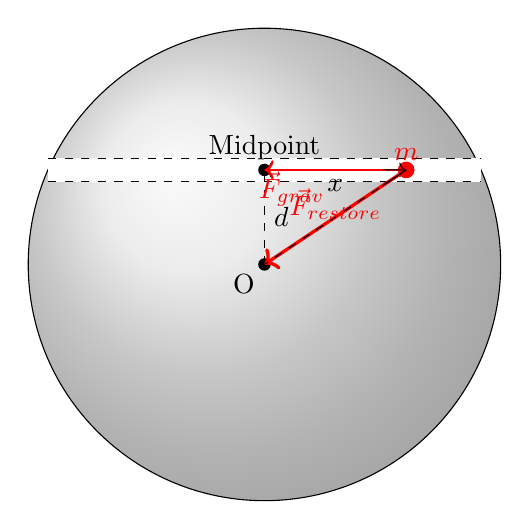
\begin{tikzpicture}[scale=1.5]
    % Earth
    \shade[ball color=gray!40!white, opacity=0.5] (0,0) circle (2cm);
    \draw (0,0) circle (2cm);
    \fill (0,0) circle (1.5pt) node[below left] {O};

    % Tunnel (Chord)
    \def\d{0.8}
    \pgfmathsetmacro{\halflen}{sqrt(4 - \d*\d)} % R=2
    \def\tunnelwidth{0.1}
    \coordinate (TL) at (-\halflen, \d + \tunnelwidth);
    \coordinate (TR) at (\halflen, \d + \tunnelwidth);
    \coordinate (BL) at (-\halflen, \d - \tunnelwidth);
    \coordinate (BR) at (\halflen, \d - \tunnelwidth);
    
    \fill[white] (BL) rectangle (TR);
    \draw[dashed] (TL) -- (TR);
    \draw[dashed] (BL) -- (BR);
    
    % Midpoint, distance d, and particle position x
    \coordinate (M) at (0, \d);
    \fill (M) circle (1.5pt) node[above] {Midpoint};
    \draw[dashed] (0,0) -- (M) node[midway, right] {$d$};
    \coordinate (P) at (1.2, \d);
    \fill[red] (P) circle (2pt) node[above] {$m$};
    \draw[<->] (M) -- (P) node[midway, below] {$x$};
    
    % Force vector and components
    \draw[->, red, very thick] (P) -- (0,0) node[midway, above left] {$\vec{F}_{grav}$};
    \draw[dashed] (P) -- (0,0);
    \draw[->, red, thick] (P) -- (M) node[midway, below=3pt] {$\vec{F}_{restore}$};
    \draw (P)++(-0.2,0) -- (P)++(-0.2,-0.133) -- (P)++(0,-0.133); % Right angle symbol
\end{tikzpicture}
\end{center}

\subsubsection*{Explanation and Solution}
Let the particle's position along the tunnel be $x$ relative to the midpoint. The particle's distance from the Earth's center is $r = \sqrt{x^2 + d^2}$. The magnitude of the gravitational force is directed towards the center and is given by $ F_{grav} = (\frac{GMm}{R^3})r$.
Only the component of this force along the tunnel causes acceleration. The restoring force is $F_{restore} = -F_{grav} \cos\phi$. From the geometry, $\cos\phi = \frac{x}{r}$.
Substituting this into the force equation:
$$F_{restore} = -\left(\frac{GMm}{R^3}\right)r \times \left(\frac{x}{r}\right) = -\left(\frac{GMm}{R^3}\right)x$$
This is a linear restoring force with the exact same effective spring constant as the tunnel through the center. The period of oscillation is therefore identical:
$$T = 2\pi\sqrt{\frac{R^3}{GM}} = 2\pi\sqrt{\frac{R}{g}}$$

\newpage
\section{Additional Example of SHM}

\subsection{Problem 5: The LC Circuit}
\subsubsection*{Problem Statement}
An ideal LC circuit consists of an inductor with inductance $L$ and a capacitor with capacitance $C$. Initially, the capacitor is fully charged with charge $Q_{max}$ and then connected to the inductor. Show that the charge on the capacitor oscillates with simple harmonic motion and determine the frequency of this electromagnetic oscillation.

\begin{center}
\begin{circuitikz}[scale=1.2]
    \draw (0,0) to[L, l=$L$] (0,2)       % 1. Bottom-left to top-left (inductor)
          -- (3,2)                       % 2. Top-left to top-right (wire)
          to[C, l=$C$, v<=$Q(t)$] (3,0) % 3. Top-right to bottom-right (capacitor)
          -- (0,0); % Changed "cycle" to the explicit coordinate                      % 4. Connects the end back to the start
        
    % Current direction arrow
    \draw[->, thick, red] (1.5,2.1) -- (1.6,2.1) node[above] {$I(t)$};
\end{circuitikz}
\end{center}

\subsubsection*{Explanation and Solution}
This system demonstrates SHM where energy oscillates between the electric field of the capacitor and the magnetic field of the inductor.
We apply Kirchhoff's Voltage Law (KVL) to the closed loop: $V_L + V_C = 0$.
The voltage across the inductor is $V_L = L \frac{dI}{dt}$, and across the capacitor is $V_C = \frac{Q}{C}$.
$$L\frac{dI}{dt} + \frac{Q}{C} = 0$$
The current $I$ is the rate of decrease of charge on the capacitor, so $I = -\frac{dQ}{dt}$, which means $\frac{dI}{dt} = -\frac{d^2Q}{dt^2}$.
Substituting this into the KVL equation:
$$L\left(-\frac{d^2Q}{dt^2}\right) + \frac{Q}{C} = 0 \implies \frac{d^2Q}{dt^2} + \left(\frac{1}{LC}\right)Q = 0$$
This is the differential equation for SHM for the charge $Q(t)$. By comparing it to the standard form, we find the angular frequency:
$$\omega = \frac{1}{\sqrt{LC}}$$
The linear frequency of the electromagnetic oscillation is $f = \omega/(2\pi)$.
$$f = \frac{1}{2\pi\sqrt{LC}}$$

\end{document}